\documentclass[final, xcolor=pdftex, dvipsnames, table, aspectratio=169, 14pt]{beamer}
\usepackage[utf8]{inputenc}
\usepackage[english]{babel}
\usepackage[T1]{fontenc}
\usepackage{droid}
\usepackage{pgf-pie}
\usepackage{hyperref}
\usetikzlibrary{decorations.pathreplacing,positioning, arrows.meta}
\frenchspacing % Don't put two spaces after periods.
\usepackage{pgfpages}

\setbeameroption{hide notes}

\setbeamerfont{note date}{size=\scriptsize}
\setbeamerfont{note title}{size=\footnotesize}
\setbeamerfont{note page}{size=\footnotesize}

\usepackage{graphicx}


\usetheme{DarkConsole}

\begin{document}

% The metadata of the presentation
\title[Worlds]{Worlds}
\subtitle[]{A Distributed MMO}
\author[]{Ryan Walker\footnote{\texttt{ryan.cjw@gmail.com}}}
\date{\today} % Replace with date of the presentation


\begin{frame}
  \maketitle
  \note{
    I'm the note from the title page.
  }
\end{frame}

\section*{I'm a hidden Section}
\begin{frame}{Table of Content} % This is the list of content with all the sections of the presentation
    \small 
    \tableofcontents
\end{frame}

\section{Identity}
\begin{frame}{Identity}
Worlds is the economic backbone for a distributed MMO. Is enables players to move digital assets and wealth throughout multiple games forming one massive congruent universe. 
\end{frame}

\begin{frame}{Identity}
\centering
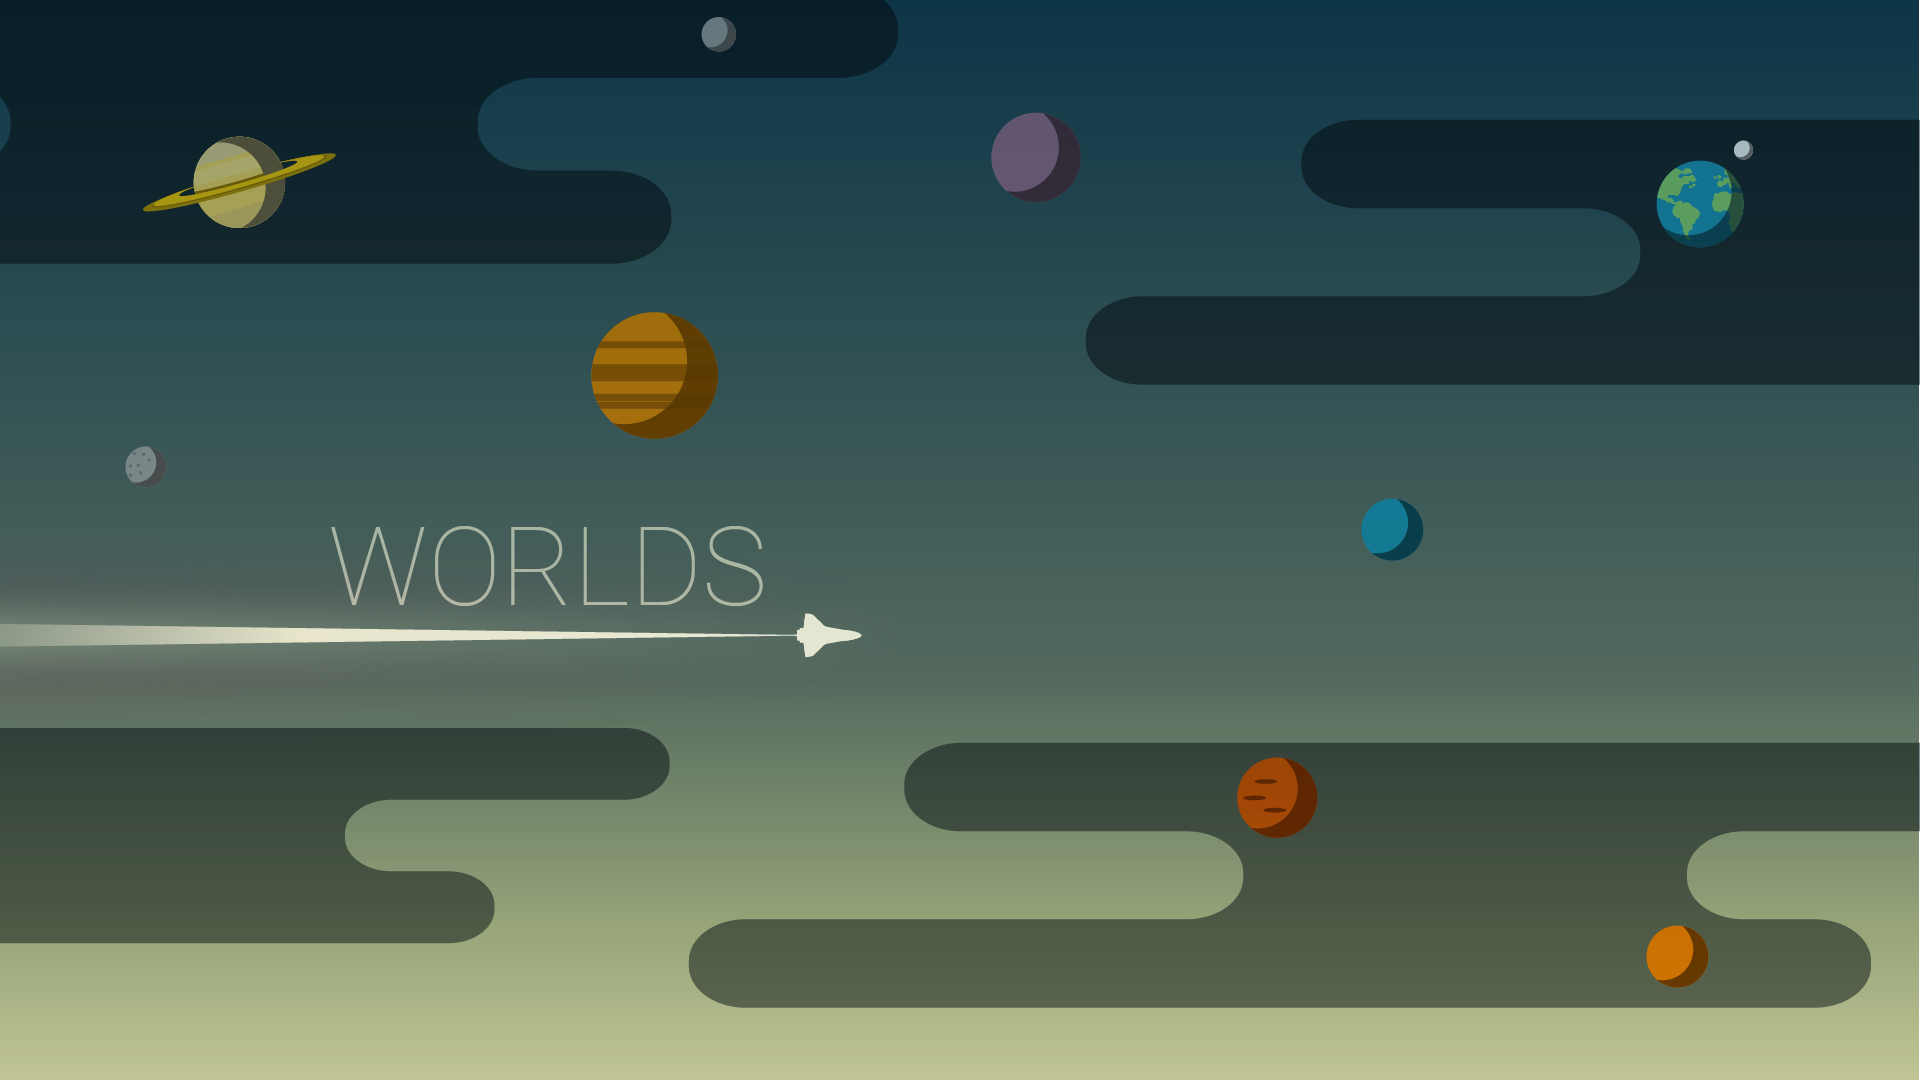
\includegraphics[scale=0.15]{Header.png} 

\textbf{Worlds} - A Distributed MMO
\end{frame}

\section{Assets}
\begin{frame}{Assets}
\href{https://www.youtube.com/watch?v=OrOZVr-j92A}{Full Stack Demo}\label{vid}
\\~\\

\href{https://github.com/Machine-Hum/Worlds/raw/master/Worlds-Whitepaper/whitepaper.pdf}{Whitepaper}
\\~\\

\href{worldsmmo.com}{Github}
\end{frame}

\section{Mission}
\begin{frame}{Mission}
Worlds is going to be the first open and scaleable infrastructure for building an unbounded MMO. Upon the completion on this platform, proper incentivisation will lead to the organic growth of the largest online game ever created.
\end{frame}

\section{Problem}
\begin{frame}{Problem}
The economy of an open world comes down to game theory. Allowing anyone to add code to a game also allows them to create unbounded resources. This creates an economic imbalance. Worlds implements a smart contract to manage the resources ensuring that digital wealth cannot be created from nothing.  
\end{frame}

\section{Solution}
\begin{frame}{Solution}
Currently there are three main components to my ecosystem, the Worlds Smart Contract, the Worlds Engine (wallet) and the Minecraft fork. These three elements have been implemented and tested to demonstrate the entire stack. 
\end{frame}

\section{Target}
\begin{frame}{Target}
To get the ball rolling, smaller communities will be targeted, I have forked and integrated an open source version on Minecraft into Worlds. The initial vision is several smaller integrated Worlds to prove out the concept. This will form a network and demonstrate the capabilities of the platform.
\end{frame}

\section{Market}
\begin{frame}{Market}
Unlike several cyrpto projects, Worlds does not suffer from the chicken and egg problem. A small implementation of ten or so Worlds maintained by independent parties would create an interesting experience. The universe will organically scale from that, funding (and later tokens) will be given to key developers at predetermined milestones.
\end{frame}

\section{Advantage}
\begin{frame}{Advantage}
My focus is full stack, by leveraging open source tech I will be able to build the game clients required to feed the initial fire. Existing projects like Worlds are relying on game developers to take a leap of faith and pour valuable development time into using their ecosystem. In the beginning coding skills shouldn't be required to create a World, just someone to host a server and create the experience. 
\end{frame}

\begin{frame}{Advantage}
My platform is 100\% open source and transparent. I want to build tools to enable my vision, and then use those tools to show people what is possible.
\end{frame}

\begin{frame}{Advantage}
Worlds is built on EOS, which has the rapid finality required for a game. 
\end{frame}

\begin{frame}{Disadvantages}
I hate this slide. Marketing is a necessary evil. I believe that strong marketing without strong tech is a fundraising mechanism. While strong marketing with strong tech is a community building mechanism. I have been focusing on the technology up until now, however in the future once I build out the tools there will be a requirement for marketing. Without funding, success will be difficult.  
\end{frame}

\section{Roadmap}

\begin{frame}{Roadmap}


\begin{center}
\begin{tikzpicture}
\draw[thick, -latex] (-0.5,0) -- (10.5,0);
%big ticks
\foreach \x in {0,4,8}
\draw (\x cm,5pt) -- (\x cm,-5pt);
%little ticks
\foreach \x in {1,2,3,5,6,7,9,10}
\draw (\x cm,3pt) -- (\x cm,-3pt);
%yr labels
\foreach \x/\descr in {0/2018,4/2019,8/2020}
\node[font=\scriptsize, text height=1.75ex,
text depth=.5ex] at (\x,0.4) {$\descr$};
%events

\draw[chartreuse, line width=4pt] (1,0) -- +(0.5,0)node[below left=2pt and 10pt,rotate=45]{\scriptsize Project Conceptulised};

\draw[chartreuse, line width=4pt] (2.25,0) -- +(0.2,0)node[below left=2pt and 10pt,rotate=45]{\scriptsize EOS Selected / Mainnet launch};

\draw[chartreuse, line width=4pt] (3,0) -- +(0.2,0)node[below left=2pt and 10pt,rotate=45]{\scriptsize Paper Complete};

\draw[chartreuse, line width=4pt] (3.75,0) -- +(0.2,0)node[below left=2pt and 10pt,rotate=45]{\scriptsize First Item Created};

\draw[chartreuse, line width=4pt] (4.2,0) -- +(0.2,0)node[below left=2pt and 10pt,rotate=45]{\scriptsize Minetest Forked};

\draw[chartreuse, line width=4pt] (5.75,0) -- +(0.2,0)node[below left=2pt and 10pt,rotate=45]{\scriptsize Wallet/Engine Functional};

\draw[chartreuse, line width=4pt] (6.5,0) -- +(0.2,0)node[below left=2pt and 10pt,rotate=45]{\scriptsize Full Stack Demo};

\draw[chartreuse, line width=4pt] (8,0) -- +(0.2,0)node[below left=2pt and 10pt,rotate=45]{\scriptsize Full Testnet Deployment};

\draw[chartreuse, line width=4pt] (9,0) -- +(0.2,0)node[below left=2pt and 10pt,rotate=45]{\scriptsize First World Deployed};

\draw[chartreuse, line width=4pt] (10,0) -- +(0.2,0)node[below left=2pt and 10pt,rotate=45]{\scriptsize Mainnet Deployment};

\end{tikzpicture}
\end{center}
\end{frame}

\section{Buisness / Token Model}
\begin{frame}{Token Cap Table}


\begin{figure}[H]
\begin{center}
\begin{tikzpicture}
\footnotesize
\pie [rotate = 180, radius=1.5, color={indigo}, explode=0.2]
{10/Kept for the team,
 40/Given to developers, 
 10/Sold to Private Investment,
 40/Community Airdrop
}
\end{tikzpicture}
\caption{Token Distribution}
\end{center}
\end{figure}
The token cap model is geared towards stimulating initial project growth within the community.
\end{frame}

\section{Fundraising}
\begin{frame}{Fundraising}

\begin{figure}[H]
\begin{center}
\begin{tikzpicture}
\footnotesize
\pie [square, radius=2.9, text=legend, after number = {k}, color={indigo, red, tomato, blue, purple, pink, orange, black}, sum=160]
{55/Personal Wage,
 10/Office Space, 
 5/Graphic Design,
 45/Contract Game Developers,
 20/UI and UX ,
 10/Concept Art,
 5/Web Development,
 10/Server Fees
}
\end{tikzpicture}
\caption{Fundraising target for year one: \textbf{\$160k}}
\label{funding}
\end{center}
\end{figure}

\end{frame}
\begin{frame}{Fundraising}
The existing development has been done on my free time. I'm looking to raise seed funding to make this my full time job. Figure \ref{funding} is the breakdown for one year of development. I'm offering 5\% of the total supply WOR for \$160k. Following the mainnet launch I will be raising a series A.
\end{frame}

\begin{frame}{Thanks}
I appreciate your consideration and hope you have gained a better understanding of my project. If you haven't watched the demo video, I would encourage you to do so. Please reach out with any questions or feedback!
\\~\\
\begin{center}
Ryan Walker - Ryan.cjw@gmail.com - \href{https://www.youtube.com/watch?v=OrOZVr-j92A}{\textcolor{blue}{Demo}}
\end{center}
\end{frame}

\end{document}
